\documentclass[a4paper]{article}
\usepackage[english]{babel}
\usepackage[utf8x]{inputenc}
% package for including graphics with figure-environment
\usepackage{graphicx}
\usepackage{hyperref}
\usepackage{amssymb}
\usepackage{amsmath}
\usepackage{mathtools}
\usepackage{graphicx}
\usepackage[export]{adjustbox}
\usepackage{tikz} 
\usepackage[ruled,vlined]{algorithm2e}
\usepackage{listings}
\usepackage{xcolor}
\usepackage{tabularx}
\lstset { %
    language=C++,
    backgroundcolor=\color{black!5}, % set backgroundcolor
    basicstyle=\footnotesize,% basic font setting
}
% colors for hyperlinks
% colored borders (false) colored text (true)
\hypersetup{colorlinks=true,citecolor=black,filecolor=black,linkcolor=black,urlcolor=black}

% package for bibliography
\usepackage[authoryear,round]{natbib}
% package for header
\usepackage[automark,headsepline]{scrlayer-scrpage}
\pagestyle{scrheadings}
\ihead[]{Multithreading Google's PageRank with CUDA}
\ohead[]{Adithya}
\cfoot[]{\pagemark} 

\begin{document}
	\title{
	\vspace{1cm}
	\Huge\textbf{ Multithreading Google's PageRank with CUDA }
	}
	
	\vspace{3cm}
	
	% if you are the only author, you might use the following
	 \author{Adithya Swaroop}	
	
	%if two authors use this
	% Insert here your name and correct mail address
	%\author{\Large \href{mailto:first.student@smail.th-koeln.de}{First Student} %\and \Large \href{mailto:second.student@smail.th-koeln.de}{Second Student}
	%\vspace{1cm}}
	
	% name of the course and module
	\date{
	\large  Course: CS6023 GPU Programming \\ 
	\vspace{0.8cm}
	\large Professor: RUPESH NASRE \\
	\vspace{1cm}
	\today
	}

	\maketitle
	\setlength{\parindent}{0pt}

\vspace{2cm}
\begin{abstract}
We use the Internet to search for information on a daily
basis. We use search engines to find out the useful
information from the vast Internet. This is possible because
the search engines are using a heuristic called PageRank. It is nothing but a value to a web page that is assigned
by a PageRanking algorithm. This algorithm scans all
possible webpages and then calculates the rank accordingly
given by a formula. Search engines show results according
these ranks, which stand for the popularity of the page. The
lower is the rank, more popular the page is. Traditional
approaches use multi-CPU architecture and this is not a
very good choice due to the communication overhead and
the low processing power of CPU compared to GPU.
Hence, designing a PageRanking algorithm efficiently
modified for parallel GPU-CPU environment that achieves
higher accuracy and consumes lesser time to evaluate the
PageRank exact rank vector even for large-scale webgraphs.


\end{abstract}
	\newpage
	\tableofcontents
	\newpage
	
\section{Introduction} % (fold)
\label{sec:introduction}
When a search is made on the Internet using a search engine, there is first a traditional
text processing part, where the aim is to find all the Web pages containing
the words of the query. Due to the massive size of the Web, the number of hits
is likely to be much too large to be of use. Therefore, some measure of quality is needed to filter out pages that are assumed to be less interesting.
When one uses a Web search engine it is typical that the search phrase is
underspecified.  
\\
\par Obviously Google uses an algorithm for ranking all the Web pages that agrees
rather well with a common-sense quality measure. Somewhat surprisingly, the ranking
procedure is based not on human judgment but on the link structure of the Web.
Loosely speaking, Google assigns a high rank to a Web page if it has in-links from
other pages that have a high rank. We will see that this self-referencing statement
can be formulated mathematically as an eigenvalue equation for a certain matrix.
% section introduction (end)

\section{Web as a Directed Graph} % (fold)
\label{sec:foundations}
Let all Web pages be ordered from 1 to $n$, and let $i$ be a particular Web page.
Then $O_i$ will denote the set of pages that $i$ is linked to, the outlinks. The number of outlinks is denoted $N_i = |O_i|$. The set of inlinks, denoted $I_i$, are the pages that have an outlink to $i$.
\\

In general, a page $i$ can be considered as more important the more inlinks
it has. However, a ranking system based only on the number of inlinks is easy to
manipulate. When you design a Web page i that (e.g., for commercial reasons)
you would like to be seen by as many users as possible, you could simply create a large number of informationless and unimportant pages that have outlinks to $i$.
To discourage this, one defines the rank of $i$ so that if a highly ranked page $j$ has an
outlink to $i$, this adds to the importance of $i$ in the following way: the rank of page
$i$ is a weighted sum of the ranks of the pages that have outlinks to $i$. The weighting
is such that the rank of a page $j$ is divided evenly among its outlinks. Translating
this into mathematics, we get
\[ r_i = \sum_{j \in I_i} \frac{r_j}{N_j}  \]
This preliminary definition is recursive, so pageranks cannot be computed directly.
Instead a fixed-point iteration might be used. Guess an initial ranking vector $r^0$.
Then iterate
\[ r_i^{(k+1)} = \sum_{j \in I_i} \frac{r_j^{(k)}}{N_j}  \]
There are a few problems with such an iteration: if a page has no outlinks, then
in the iteration process it accumulates rank only via its inlinks, but this rank is
never distributed further. Therefore it is not clear if the iteration converges. We
will come back to this problem later.
More insight is gained if we reformulate as an eigenvalue problem for
a matrix representing the graph of the Internet. Let $Q$ be a square matrix of
dimension $n$. Define
\[
    Q_{ij} = \begin{dcases}
    \frac{1}{N_j}   &  \mathrm{if \ there \ is \ a \ link\ from\ j\ to\ i}\                   \\
    0   &  \mathrm{otherwise}        \\
      \end{dcases}
    \]
This means that row $i$ has nonzero elements in the positions that correspond to
inlinks of $i$. Similarly, column $j$ has nonzero elements equal to $ N_j$ in the positions
that correspond to the outlinks of $j$, and, provided that the page has outlinks, the
sum of all the elements in column $j$ is equal to one. Suppose a page $i$ has no outlinks, all elements in $i^{th}$ column will be 0.  
\\
For below graph, 
\begin{center}

\begin{tikzpicture}[node distance={30mm}, thick, main/.style = {draw, circle}] 
\node[main] (1) {$1$}; 
\node[main] (2) [ right of=1] {$2$}; 
\node[main] (3) [ right of=2] {$3$}; 
\node[main] (4) [below of=1] {$4$}; 
\node[main] (5) [ right of=4] {$5$}; 
\node[main] (6) [right of=5] {$6$}; 
\draw[->] (1) -- (2);
\draw[->] (2) -- (1);
\draw[->] (2) -- (3);
\draw[->] (1) -- (4);
\draw[->] (1) -- (5);
\draw[->] (2) -- (5); 
\draw[->] (2) -- (3); 
\draw[->] (3) -- (6); 
\draw[->] (5) -- (3); 
\draw[->] (5) -- (4); 
\draw[->] (5) -- (6); 
\draw[->] (6) -- (5); 
\draw[->] (6) -- (3); 

\end{tikzpicture} 
\end{center}
Corresponding matrix becomes
$$
Q = \begin{bmatrix}
0 & \frac{1}{3} & 0 & 0 & 0 & 0\\
\frac{1}{3} & 0 & 0 & 0 & 0 & 0\\
0 & \frac{1}{3} & 0 & 0 & \frac{1}{3} & \frac{1}{2}\\
\frac{1}{3} & 0 & 0 & 0 & \frac{1}{3} & 0\\
\frac{1}{3} &\frac{1}{3} & 0 & 0 & 0 & \frac{1}{2}\\
0 & 0 & 1 & 0 & \frac{1}{3} & 0
\end{bmatrix}$$
Since page 4 has no outlinks, the corresponding column is equal to zero.
Obviously, the above definition is equivalent to the scalar product of row $i$
and the vector $r$, which holds the ranks of all pages. We can write the equation in matrix form,
$$ \lambda r = Q r,\ \lambda = 1$$
i.e., $r$ is an eigenvector of $Q$ with eigenvalue $\lambda$ = 1. It is now easily seen that the
iteration mentioned above is equivalent to
$$ \lambda r^{(k+1)} = Q r^{(k)},\ k= 0, 1...$$
which is the \textbf{power method} for computing the eigenvector. However, at this point
it is not clear that pagerank is well defined, as we do not know if there exists an
eigenvalue equal to 1. It turns out that the theory of Markov chains is useful in the
analysis.
\newpage
\section{Random Walk and Markov Chains} % (fold)
\label{sec:section_about_quotations}
There is a random walk interpretation of the pagerank concept. Assume that a
surfer visiting a Web page chooses the next page among the outlinks with equal
probability. Then the random walk induces a Markov chain . A
Markov chain is a random process in which the next state is determined completely
from the present state; the process has no memory. The transition matrix of the
Markov chain is $Q_T$ . (Note that we use a slightly different notation than is common
in the theory of stochastic processes.)
The random surfer should never get stuck. In other words, our random walk
model should have no pages without outlinks. (Such a page corresponds to a zero
column in $Q$.) Therefore the model is modified so that zero columns are replaced
with a constant value in all positions. This means that there is equal probability to
go to any other Internet page. Define the vectors

\[
    d_{j} = \begin{dcases}
    1   &  \mathrm{if}\ N_j = 0                   \\
    0   &  \mathrm{otherwise}        \\
      \end{dcases}
    \]
for $j = 1, . . . , n,$ and
$$e = \begin{pmatrix}
  1\\ 
  1\\
  .\\
  .\\
  1
\end{pmatrix} \in \mathbb{R}^n$$
The modified matrix is defined
$$P = Q + \frac{1}{n}ed^T$$
With this modification the matrix P is a \textbf{proper column-stochastic matrix}. It has
nonnegative elements, and the elements of each column sum up to 1. The preceding
statement can be reformulated as follows.
$$e^TP = e^T$$

So the matrix in the previous graph modifies to 
$$
P = \begin{bmatrix}
0 & \frac{1}{3} & 0 & \frac{1}{6} & 0 & 0\\
\frac{1}{3} & 0 & 0 & \frac{1}{6} & 0 & 0\\
0 & \frac{1}{3} & 0 & \frac{1}{6} & \frac{1}{3} & \frac{1}{2}\\
\frac{1}{3} & 0 & 0 & \frac{1}{6} & \frac{1}{3} & 0\\
\frac{1}{3} &\frac{1}{3} & 0 & \frac{1}{6} & 0 & \frac{1}{2}\\
0 & 0 & 1 & \frac{1}{6} & \frac{1}{3} & 0
\end{bmatrix}
$$
We would like to define the pagerank vector as a unique
eigenvector of P with eigenvalue 1,
$$Pr = r.$$
The eigenvector of the transition matrix corresponds to a stationary probability
distribution for the Markov chain. The element in position $i$, $r_i$, is the probability
that after a large number of steps, the random walker is at Web page $i$. However,
the existence of a unique eigenvalue with eigenvalue 1 is still not guaranteed. To
ensure uniqueness, the matrix must be \textbf{irreducible}.

To illustrate the concept of reducibility, we give an example of a
link graph that corresponds to a \textit{reducible} matrix:

\begin{center}

\begin{tikzpicture}[node distance={30mm}, thick, main/.style = {draw, circle}] 
\node[main] (1) {$1$}; 
\node[main] (2) [ right of=1] {$4$}; 
\node[main] (3) [ right of=2] {$5$}; 
\node[main] (4) [below of=1] {$2$}; 
\node[main] (5) [ right of=4] {$3$}; 
\node[main] (6) [right of=5] {$6$}; 
\draw[->] (1) -- (4);
\draw[->] (4) -- (1);
\draw[->] (1) -- (5);
\draw[->] (5) -- (1);
\draw[->] (4) -- (5);
\draw[->] (5) -- (4); 
\draw[->] (2) -- (1); 
\draw[->] (2) -- (3); 
\draw[->] (3) -- (6); 
\draw[->] (6) -- (3); 


\end{tikzpicture} 
\end{center}
A random walker who has entered the left part of the link graph will never get
out of it, and similarly will get stuck in the right part.
The directed graph corresponding to an irreducible matrix is \textbf{strongly connected}:
given any two nodes $(N_i,N_j )$, in the graph, there exists a path leading
from $N_i$ to $N_j$ .\\

Given the size of the Internet, we can be sure that the link matrix P is reducible,
which means that the pagerank eigenvector of $P$ is not well defined. To
ensure irreducibility, i.e., to make it impossible for the random walker to get trapped
in a subgraph, one adds, artificially, a link from every Web page to all the others. In
matrix terms, this can be made by taking a convex combination of P and a rank-1
matrix,
$$A = \alpha P + (1- \alpha)\frac{1}{n}ee^T$$
for some $\alpha$ satisfying $0 \leq \alpha 1$. It is easy to see that the matrix A is column-stochastic:
$$e^TA = \alpha e^TP + (1 − \alpha)\frac{1}{n}e^T ee^T = \alpha e^T + (1 − \alpha)e^T = e^T$$
The random walk interpretation of the additional rank-1 term is that in each time
step the surfer visiting a page will jump to a random page with probability $1 − \alpha$
(sometimes referred to as teleportation).
We now see that the pagerank vector for the matrix $A$ is well defined.

\section{Power Method for PageRank computation}
We want to solve the eigenvalue problem
$$Ar = r$$
where $r$ is normalized 
$||r||_1 = 1$.
 In this section we denote the sought eigenvector by
$t_1$. Dealing with stochastic matrices and vectors that are probability distributions,
it is natural to use the 1-norm for vectors. Due to the sparsity and
the dimension of A (of the order billions), it is out of the question to compute the
eigenvector using any of the standard methods on applying orthogonal transformations to
the matrix. The only viable method so far is the power method.
Assume that an initial approximation $r^{(0)}$ is given. The power method is given
in the following algorithm.\\
\begin{algorithm}[H]
\SetAlgoLined

 \For{($k$  = 1, 2, . . . until convergence)}{
  $q^{(k)} = Ar^{(k-1)}$\\
  $ r^{(k)} = q^{(k)}/||q^{(k)}||_1$
 }
 \caption{The power method for $Ar = \lambda r$}
\end{algorithm}

\section{Multi-threading Power Method}
C++ code for Power Method looks like this.

\begin{verbatim}
void power_method(float **graph, float *r, int n ){
    int max_iter = 1000; float eps = 0.000001;
    float* r_last = (float*) malloc(n * sizeof(float));
    
    for(int i = 0; i< n; ++i){
        r[i] = (1/(float)n);
    }

    while(max_iter--){
        for(int i = 0; i< n; ++i){
            r_last[i] = r[i];
        }
        for(int i = 0; i< n; ++i){
            float sum = 0.0;
            for (int j = 0; j< n; ++j){
                sum += r_last[j] * graph[i][j];
            }
            r[i] = sum;
        }

        for(int i = 0; i< n; ++i){
            r_last[i] -= r[i];
        }

        if(norm(r_last, n) < eps){
            return;
        }
    }
    return;
}
\end{verbatim}
\newpage
\textcolor{red}{The complexity of this algorithm is $O(n^3)$, which will be very heavy to handle computationally for large scale web graph with 100,000 nodes. We can also observe that most of those loops in outermost while loop are iterating through every node. We can reduce the computational burden here by paralleling that operation. There is no sight of any data race, thread divergence too. Also, adjacent threads access adjacent memory locations in every case and Degree of coalescing is maximum.
So, we can remove the suppress the for loops by paralleling them. Kernels after paralleling looks like this.}
\begin{verbatim}
__global__ void initialize_rank(float* gpu_r, int n){
    int id = blockIdx.x * blockDim.x + threadIdx.x;

    if(id < n){
        gpu_r[id] = (1/(float)n);
    }
}

__global__ void store_rank(float* gpu_r,float* gpu_r_last, int n){
    int id = blockIdx.x * blockDim.x + threadIdx.x;

    if(id < n){
        gpu_r_last[id] = gpu_r[id];
    }
}

__global__ void matmul(float* gpu_graph, float* gpu_r, float* gpu_r_last, int n){
    int id = blockIdx.x * blockDim.x + threadIdx.x;

    if(id < n){
        float sum = 0.0;

        for (int j = 0; j< n; ++j){
            sum += gpu_r_last[j] * gpu_graph[id* n + j];
        }

        gpu_r[id] = sum;
    }
}

__global__ void rank_diff(float* gpu_r,float* gpu_r_last, int n){
    int id = blockIdx.x * blockDim.x + threadIdx.x;

    if(id < n){
        gpu_r_last[id] = abs(gpu_r_last[id] - gpu_r[id]);
    }
}
\end{verbatim}
For sorting the final rank vector returned after power method, we can use \textbf{thrust::sort()} instead of normal \textbf{std::sort()}, even this saves us time in case of large scale network graphs.

\section{Experiments}
\subsection{Time vs Number of nodes}
\begin{tabularx}{\textwidth} { 
  | >{\raggedright\arraybackslash}X 
  | >{\centering\arraybackslash}X 
  | >{\centering\arraybackslash}X 
  | >{\raggedleft\arraybackslash}X | }
 \hline
  No: of nodes & sequential & parallel & speedup \\
 \hline
100  &  405 &  593 &   0.68 \\
   \hline
200  & 6556  & 2152  &  3.04  \\ 
  \hline
400  &  3462 & 936  &  3.69  \\ 
  \hline
800  &  22785 & 2356  &  9.67  \\
   \hline
1000  &  2972898 & 104831  &  28.35  \\
   \hline
 5000 & 69266776  &  816446 &  84.83  \\
    \hline
10000 & 68519880  & 755148  &  90.73  \\
    \hline
16000 & 26509166  & 626986  &  42.28  \\
\hline
\end{tabularx}\\

\begin{figure}[h]
    \centering
    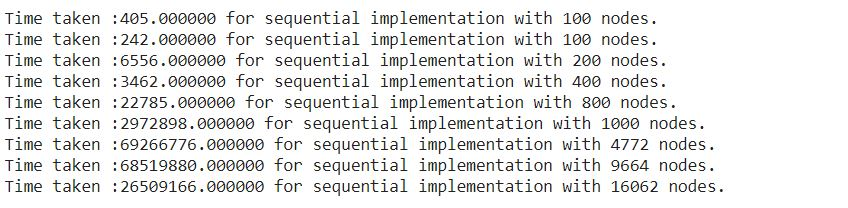
\includegraphics[width=1\textwidth]{PageRank/img/Capture.JPG}
    
\end{figure}
\begin{figure}[h]
    \centering
    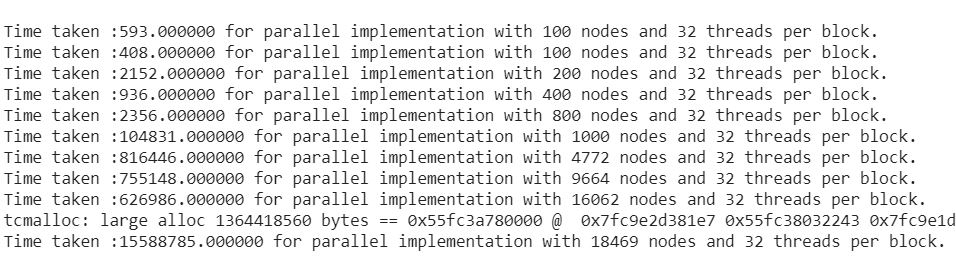
\includegraphics[width=1\textwidth]{PageRank/img/Capture2.JPG}
 
\end{figure}

We can observe that there is no trend with respect to number of nodes. Performance of PageRank algorithm also depends on how nodes are connected too. If it's a perfectly reducible matrix, algorithm converges quickly, but if that's not the case, algorithm doesn't converge even after 100 iterations.

\subsection{Time vs Number of threads in a block}
\begin{figure}[h]
    \begin{center}
    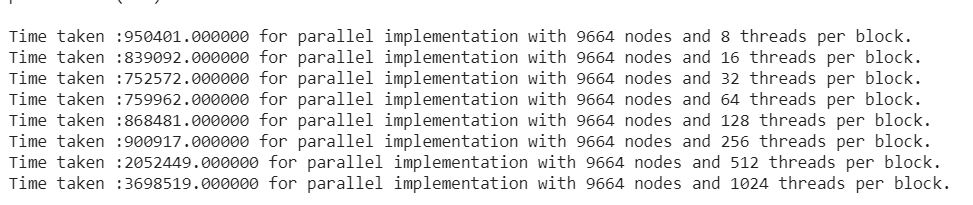
\includegraphics[width=1\textwidth]{PageRank/img/Capture8.JPG}
    \end{center}
\end{figure}
As number of threads in a block increases, performance decreases.
\subsection{Top Pages}
Here are the top 3 nodes after computation of power method sequentially and parallelly.
\begin{figure}[h]
    \begin{center}
    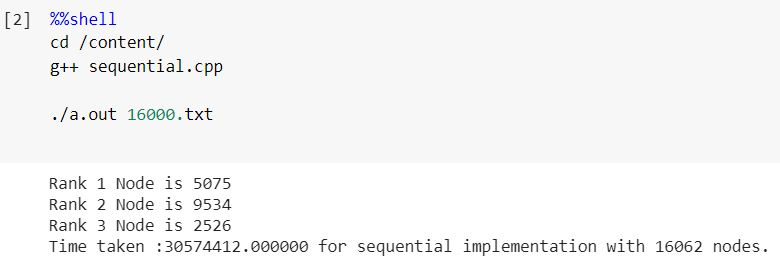
\includegraphics[width=1\textwidth]{PageRank/img/Capture3.JPG}
    \end{center}
\end{figure}
\begin{figure}[h]
    \begin{center}
    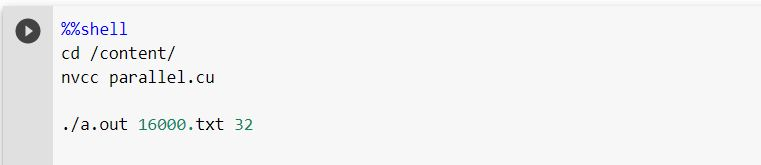
\includegraphics[width=1\textwidth]{PageRank/img/Capture4.JPG}
    \end{center}
\end{figure}
\begin{figure}[h]
    \begin{center}
    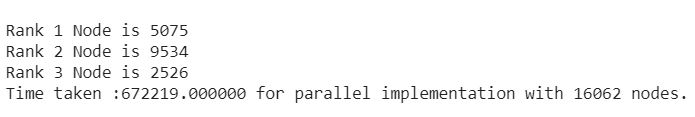
\includegraphics[width=1\textwidth]{PageRank/img/Capture5.JPG}
    \end{center}
\end{figure}

\section{New Idea : TweetRank}
Above all experiments are conducted on \href{http://networkrepository.com/web.php}{\textcolor{blue}{web network datasets}}. But, now let's try them on \href{http://networkrepository.com/rt-pol.php}{\textcolor{blue}{twitter retweet network dataset.}} \\

Let us hope that just like in case of ranking pages from web graphs, we can rank best tweets for twitter search. If many users retweets an user's tweet, it may be important. And if that user retweets another tweet, it contains information which is not in his tweet, so even it is slightly important. Let us run our algorithm on that dataset.
\begin{figure}[h]
    \begin{center}
    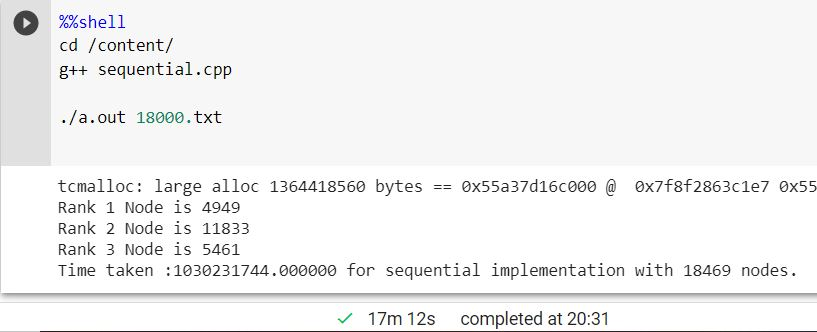
\includegraphics[width=1\textwidth]{PageRank/img/Capture6.JPG}
    \end{center}
\end{figure}
\begin{figure}[h]
    \begin{center}
    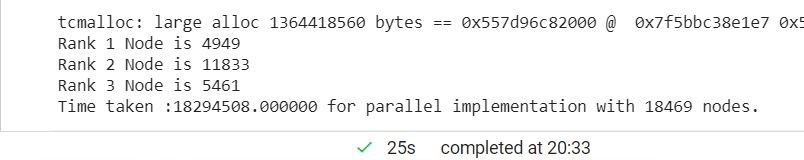
\includegraphics[width=1\textwidth]{PageRank/img/Capture7.JPG}
    \end{center}
\end{figure}
\\

Though we got results (next page) and a good speedup (25 s vs 17 min), we should not suppress the fact that sequential implementation took 17 min to run, which is very abnormal compared to other datasets. We can observe that it did not converge so our hypothesis of ranking \textbf{may be wrong}. Retweet network graph may not be reducible. 

\section{References}
\begin{itemize}
    \item \href{https://github.com/priyendumori/Parallel-implementation-of-PageRank}{\textcolor{blue}{Parallel-implementation-of-PageRank}}
    \item \href{https://hippocampus-garden.com/pagerank/#:~:text=The%20power%20method%20is%20a,M%20to%20any%20initial%20vector.}{\textcolor{blue}{PageRank Explained: Theory, Algorithm, and Some Experiments}}
    \item Book: Matrix Methods in Data Mining and Pattern Recognition
    \item \href{http://www.cs.cornell.edu/courses/cs685/2002fa/data/gr0.California}{\textcolor{blue}{Real-World Dataset}}
    \item \href{https://github.com/JiaoMaWHU/CudaPageRank/tree/master/data}{\textcolor{blue}{More data}}
    \item \href{http://networkrepository.com/web.php}{\textcolor{blue}{Web network datasets}}
    \item \href{http://networkrepository.com/rt-pol.php}{\textcolor{blue}{Twitter Retweet network dataset}}
\end{itemize}
\end{document}